%  LaTeX support: latex@mdpi.com 
%  In case you need support, please attach all files that are necessary for compiling as well as the log file, and specify the details of your LaTeX setup (which operating system and LaTeX version / tools you are using).

% You need to save the "mdpi.cls" and "mdpi.bst" files into the same folder as this template file.

%=================================================================
\documentclass[soilsystems,article,submit,moreauthors,pdftex,10pt,a4paper]{Definitions/mdpi} 

% If you would like to post an early version of this manuscript as a preprint, you may use preprint as the journal and change 'submit' to 'accept'. The document class line would be, e.g., \documentclass[preprints,article,accept,moreauthors,pdftex,10pt,a4paper]{mdpi}. This is especially recommended for submission to arXiv, where line numbers should be removed before posting. For preprints.org, the editorial staff will make this change immediately prior to posting.

%
%--------------------
% Class Options:
%--------------------

%----------
% submit
%----------
% The class option "submit" will be changed to "accept" by the Editorial Office when the paper is accepted. This will only make changes to the frontpage (e.g., the logo of the journal will get visible), the headings, and the copyright information. Also, line numbering will be removed. Journal info and pagination for accepted papers will also be assigned by the Editorial Office.
%------------------
% moreauthors
%------------------
% If there is only one author the class option oneauthor should be used. Otherwise use the class option moreauthors.
%---------
% pdftex
%---------
% The option pdftex is for use with pdfLaTeX. If eps figures are used, remove the option pdftex and use LaTeX and dvi2pdf.

%=================================================================
\firstpage{1} 
\makeatletter 
\setcounter{page}{\@firstpage} 
\makeatother
\pubvolume{xx}
\issuenum{1}
\articlenumber{5}
\pubyear{2018}
\copyrightyear{2018}
%\externaleditor{Academic Editor: name}
\history{Received: date; Accepted: date; Published: date}
%\updates{yes} % If there is an update available, un-comment this line

%% MDPI internal command: uncomment if new journal that already uses continuous page numbers 
%\continuouspages{yes}

%------------------------------------------------------------------
% The following line should be uncommented if the LaTeX file is uploaded to arXiv.org
%\pdfoutput=1

%=================================================================
% Add packages and commands here. The following packages are loaded in our class file: fontenc, calc, indentfirst, fancyhdr, graphicx, lastpage, ifthen, lineno, float, amsmath, setspace, enumitem, mathpazo, booktabs, titlesec, etoolbox, amsthm, hyphenat, natbib, hyperref, footmisc, geometry, caption, url, mdframed, tabto, soul, multirow, microtype, tikz

%=================================================================
%% Please use the following mathematics environments: Theorem, Lemma, Corollary, Proposition, Characterization, Property, Problem, Example, ExamplesandDefinitions, Hypothesis, Remark, Definition
%% For proofs, please use the proof environment (the amsthm package is loaded by the MDPI class).

%=================================================================
% Full title of the paper (Capitalized)
\Title{Topographic control on soil function evaluation -  a case study from South Tyrol}

% Author Orchid ID: enter ID or remove command
\newcommand{\orcidauthorA}{0000-0002-3293-9691} % Add \orcidA{} behind the author's name
%\newcommand{\orcidauthorB}{0000-0000-000-000X} % Add \orcidB{} behind the author's name

% Authors, for the paper (add full first names)
\Author{Fabian Ernst Gruber $^{1,*,\dagger,\ddagger}$\orcidA{}, Elisabeth Schaber $^{1,\ddagger}$, Jasmin Baruck $^{1,\ddagger}$ and Clemens Geitner $^{1,}$}

% Authors, for metadata in PDF
\AuthorNames{Firstname Lastname, Firstname Lastname and Firstname Lastname}

% Affiliations / Addresses (Add [1] after \address if there is only one affiliation.)
\address[1]{%
$^{1}$ \quad University of Innsbruck, Institute of Geography; geographie@uibk.ac.at\\}

% Contact information of the corresponding author
\corres{Correspondence: fabian.gruber@ages.at}

% Current address and/or shared authorship
\firstnote{Current address: Austrian Agency for Health and Food Security} 
\secondnote{These authors contributed equally to this work.}
% The commands \thirdnote{} till \eighthnote{} are available for further notes

%\simplesumm{} % Simple summary

%\conference{} % An extended version of a conference paper

% Abstract (Do not insert blank lines, i.e. \\) 
\abstract{}

% Keywords
\keyword{soil function evaluation; digital terrain analysis; support vector machine classification)}

% The fields PACS, MSC, and JEL may be left empty or commented out if not applicable
%\PACS{J0101}
%\MSC{}
%\JEL{}


%\datasetlicense{license under which the data set is made available (CC0, CC-BY, CC-BY-SA, CC-BY-NC, etc.)}

%\setcounter{secnumdepth}{4}
%%%%%%%%%%%%%%%%%%%%%%%%%%%%%%%%%%%%%%%%%%
\begin{document}


\section{Introduction}
Information on soil, a, at least from a human time perspective, non-renewable ressource, is of increasing importance given erosion, soil degradation and soil sealing. It is necessary to know where and where not certain practises are applicable and to adjust land-use planning appropriately. Accordingly, soil function evaluation is an invaluable tool for the future.\newline

\cite{Haslmayr2016} and further literature
\newline

In this study, we present the soil evaluation tool \emph{Soil Evaluation for Planning Procedures (SEPP)} and investigate topographic and parent material control of the different soil functions by applying a cross-validated machine learning approach based on availible soil pit information in the Oltradige/\"{U}beretsch region of the Autonomous Province Bolzano - South Tyrol. 

The main aim of the study is 


\section{Materials and Methods}

\subsection{Study area and soil data}

\subsection{SEPP - Soil Evaluation for Planning Procedures}
The software SEPP currently computes a soil function evaluation based on soil pit descriptions. It requires that the pit descriptions are performed following the Austrian Soil classification  \citep{Nestroy2000,Nestroy2011} and related mapping manuals. The minimum  soil profile site characteristics are local slope, thickness of organic horizons, soil depth, groundwater table, soil parent material, soil type, humus form, altitudinal zone, moisture level and land use.For each horizon, the minimum characteristics necessary for computing the soil function are the master horizon designation, depth, pH value, proportion of the dominant soil structure type and class membership with regard to carbonate content, soil texture, organic content, abundance of rock fragments, bulk density, soil structure. These class attributes can be substituted by exact values if available. The soil functions, for which 15 different potentials are computed, are  \emph{habitat for living organisms} (specifically the potential as habitat for drought-tolerant species, moisture tolerant species, soil organisms and crops),  \emph{infiltration and drainage regulation} (minimum, average and heavy precipitation retention capacity as well as groundwater reformation rate), \emph{natural soil fertility} as well as \emph{filter and buffer for pollutants} (heavy metal, organic, acidifying and water-soluble). The result is a grade between 1 and 5 for each soil function potential, with 1 signifying a high potential and 5 a low one.

\paragraph{Potential as a habitat for drought-tolerant species} 
Both this potential and the following potential as a habitat for moisture-tolerant species are performed based on modifications of the approaches decribed by \cite{BAYGLA2003} and \cite{Lehmann2008}.
The evaluation of a soil's potential  as a habitat for drought-tolerant species is based on the parameters land use, soil type and available field capacity. While the first two parameters are applied to distinguish especially suited (ruderal locations and corresponding soil types) or unsuited (mire deposits and soil types commonly found on these) sites, the latter is used to grade those soil profile sites showing the remaining landuse and soil type combinations. 
\paragraph{Potential as a habitat for moisture-tolerant species}
This potential is evaluated similarly to the the one for drought-tolerant species, in that specific soil types, e.g. Gleysols, are attributed specific grades. In addition, the depth of the groundwater table is used to distinguish sites with high potential, and the available field capacity is used to differentiate even further.
\paragraph{Habitat for soil organisms}
This potential is evaluated according to \cite{Beylich2005} with some minor adaptions. In this framework, a number of species groups are used as indicators for the composition of soil life, with emphasis on earth worms (Lumbricidae) as they are influential on soil structure and bioturbation. This method is based on the relationship between soil organism communities and a number of abiotic soil parameters. Specifically, one of 14 possible soil organism communities, which are the basis for the grade awarded to a site, is attributed to a site according to a classification tree applying the parameters pH, moisture level, land use and soil texture.
\paragraph{Potential for agricultural production}
The assessment of the potential for agricultural production is performed according to the method proposed in the framework TUSEC-IP \citep{Lehmann2008} by an accumulative rating of five criteria. The criteria \emph{general conditions of the profile site} is rated based on soil depth, topsoil aggregate structure and topsoil as well as subsoil bulk density. While the criteria \emph{water supply} is based on available field capacity and the depth of the groundwater table, the grade for \emph{air supply} is derived from air capacity and for \emph{nutrient supply} the alkaline cation exchange capacity is regarded. The \emph{climate} criteria is derived from the mean annual temperature of the growing season if available, or else replaced by proxy values such as mean annual temperature or altitudinal zone. The combination of the grades of the individual criteria for agricultural production leads to an overall grade that is then adjusted for the slope gradient of the location.
\paragraph{Average and minimum precipitation retention capacity}
Following a modified version of the procedures presented by \cite{LUBW1995} and \cite{BAYGLA2003}, this potential is assessed by combining the permeability coefficient (using either the average value of the soil profile or the minimum value) with the water storage capacity. For more or less planar areas, the water storage capacity is regarded as  the sum of the usable field capacity and the air capacity, whereas for steeper slopes only the former parameter is used. Additionally, permeability coefficient and water storage capacity is considered only for soil horizons not linked to contact with groundwater or stagnant water.
\paragraph{Retention capacity for heavy precipitation events}
 The evaluation of this soil potential is a modfied version of the scheme proposed by \citep{Lehmann2008}. It differs from the agerage precipitation retention capacity by being based on the assumption that flooding hazards are greatest when soils are already saturated with water, and therefore only the air storage capacity is considered for retention. This retention volume is then compared to the design rainfall event under consideration of the infiltration rate.
\paragraph{Quality of groundwater reformation}
Also following \citep{Lehmann2008}, this potential is assessed using the same parameters as the precipitation capacity but considers the assumption that very quick infiltration leads to an increase of pollutants in the groundwater. In the same reasoning, soil types linked to groundwater or locations with high groundwater table are given poorer grades.
\paragraph{Potential for providing nutrients for plants}
Adhering to \citep{Mueller2011}, the assessment of this potential uses the parameter alkaline cation exchange capacity. As this is only a coarse approximation, this potential is not differentiated into five, but only three classes (poor, average and high potential).
\paragraph{Potential as a CO2 sink}
By applying a modified version of the rating proposed by \cite{Gerstenberg2005}, selected land uses, especially forests, are awarded good grades, whereas other landuses are graded based on the amount of organic matter, summed up over all soil horizons.
\paragraph{Potential for retention of heavy metals}
In this assessment, the ability to bind cadmium is used as a proxy for other heavy metals. Based on modifications of the procedures proposed by \cite{AGBoden2000} and \cite{BAYGLA2003},in a first step this ability is evaluated for different pH-values for sandy soils with little organic content, and later adjusted with regard to organic matter content and soil texture as a proxy for clay content.
\paragraph{Potential for transforming organic contaminants}
As organic pollutants are generally transformed by soil organisms, this potential can be essentially assessed by rating the living conditions for soil micro-organisms. Consequently, the parameters which contribute to the rating procedure based on \cite{LUBW1995}  are topsoil organic matter content, topsoil clay content and the average topsoil pH-value. In a first step, microbial activity is estimated based on humus form and pH-value, and then the potential for transformation is further differentiated based on organic matter and clay content.
\paragraph{Potential as  filter and buffer for organic contaminants}
As the evaluation of a representative contaminant (such as cadmium for heavy metals) is not feasible for organic contaminants due to their variety, this potential is assessed by estimating a mean binding capacity for organic pollutants using organic matter and clay content for the fine material contained within a soil profile.
\paragraph{Potential for retention of water-soluble contaminants}
For the assessment of the potential for retention of water-soluble pollutants, with emphasis on nitrate, the yearly seepage rate is calculated based on mean precipitation, mean evaporation and an estimate of surface run-off derived from soil texture. The grade for this potential is rewarded based on the annual exchange rate of soil water by comparing seepage volume with field capacity.
\paragraph{Potential as buffer for acidic contaminants}
The potential buffer capacity is evaluated according to \cite{BAYGLA2003} by considering the alkaline cation exchange capacity and the carbonate content of the mineral horizons on the one hand, and estimating the buffer capacity of the organic layer from its humus form and thickness on the other hand.
\subsection{The predictor variable set:terrain parameters and landform classification}
Terrain parameters, i.e. variables derived from performing calculations on digital terrain models  (DTM) have long played an important role in modeling parameters or processes associated with geomorphology, soil, natural hazards, or habitat modeling, to just name a few scientific fields. An overview of terrain parameters, their calculation, and application can be found for instance in \cite{Gallant2000, Olaya2009}. While a wide variety of different terrain parameters are available, the presented study concentrates on simple local terrain parameters as well as an automated landform classification algorithm. For the former group of parameters, slope and a variety of curvature measures (planar, profile, cross-sectional, and tangential) were computed at varying window sizes using the GRASS GIS 7 \citep{GRASS} module r.param.scale. With regard to landforms,  \cite{Gruber2017} showed in their comparison of automated landform classifications and the topographic description of soil pit sites,that the r.geomorphon algorithm by \cite{Jasiewicz2013} is a valuable tool for use in soil survey. It uses pattern recognition based on line-of-sight calculations to classify each grid cell of a digital terrain model as one of 10 possible landforms (Figure~\ref{fig:geomorphonlegend}). These landform classifications were performed considering modifications of the two parameters search window size and flatness threshold. While the former parameter is responsible for how many surrounding grid cells are considered when performing the line-of-sight calculations, thus influencing the scale at which the landforms are computed, the latter represents the slope angles up to which a grid cell is regarded to be flat. \cite{Gruber2017} showed that investigating the result of varying flatness thresholds is of interest especially in an Alpine environment.
 \begin{figure}[ht!]
\includegraphics[width=\textwidth,angle=0]{legende_geomorphons_cropped.pdf}
\caption{The r.geomorphon algorithm  classifies every grid cell of a given digital terrain model as one of these 10 landforms based on line-of-sight calculations (figure based on \cite{Jasiewicz2013})}
\label{fig:geomorphonlegend}
\end{figure}
\subsection{Statistical learning and variable selection procedure}
Support vector machine (SVM) classification is a statistical learning approach first described by \cite{Cortes1995}. Its classification algorithm computes a hyper-plane that best separates different classes by concentrating on those data points of both classes (support vectors) which are within a certain margin of the hyperplane. In this process, SVM classification also allows some points to be on the \emph{wrong} side of the hyperplane, a behavior that can be addressed with the tuning parameter c.  By applying a radial kernel this linear binary classification can be extended to the non-linear case. A majority vote system then further allows application of SVM-classification for multiple classes. In the presented study, the SVM-algorithm as implemented in the package \emph{e1071} \citep{Meyer2014} of the open source statistical computing environment R \citep{cran2014} was used.

A forward step-wise feature selection procedure based on 10-fold cross-validation using SVM classification was applied to select the best parameter or parameter combination for each soil function or potential. Cross-validation  (5-fold) was also applied to the entire feature selection procedure, meaning that after partitioning the data set into five sets, one part is set aside for validation to be used after the feature selection procedure has been carried out with the four remaining parts used for the model fitting. The usefulness of additional parameters in the model were evaluated using the \emph{one-standard-error-rule} \citep{James2013}, meaning that the number of explanatory variables was seen sufficient if the improvement through adding more explanatory variables did not exceed one standard error of the predictions. As the selection process at times revealed a number of parameter combinations leading to comparable cross-validated accuracies as well as showing a wide range of these values, the different parameter combinations were then compared by performing the 10-fold CV 100 times, each time with 10 different, random partitions. The median values and distribution of accuracy values were compared, as were the confusion matrices based on the whole data set, where the final modeled soil function classes were attributed using the majority vote of the 100 predictions.  Additionally, the models resulting from different parameter combinations  were used to predict the soil function potentials for the entire study area and visualized as maps to examine how they performed spatially.

\subsection{Post-feature selection workflow}
After the feature selection procedure, the classes, consisting of soil pits with the same grade for a given potential, were analyzed with regard to the chosen terrain parameters or landform classification. This was performed with the original classes, but also with the projected classes in order to investigate the effect of the different parameters on the output of the model based on the support vector machine classification. An example of such a box plot analysis of the distribution of terrain parameters is given in Figure~\ref{fig:slope_agriculture}. This analysis also gives insight into certain aspects explaining user's and producer's reliability as derived from evaluation of the confusion matrix based on the 100 prediction runs.  User's accuracy gives the percentage of correctly classified members of a class with regard to the total number of members in the respective reference class, which in this study is the classification performed by the SEPP tool. Producer's reliability on the other hand relates the correctly classified members of a given class to the total number of members predicted by the model.
If a landform classification was chosen as best suited to distinguish between soil profile site locations of different grades for a potential, bar plots instead of box plots were applied to investigate and visualize the model output. For each soil function grade, the distribution of the 10 landforms was plotted in order to conceive how the dominance of different landforms changed for the different grades, and how the SVM model attributed the projected grades to different landforms. Figure~\ref{fig:transformorganic} shows such a plot for the soil function of transforming organic contaminants.

\section{Results}
The soil function grades for each of the 15 potentials was calculated for each of the 108 soil profile pits in the study area with the SEPP application. Figure \ref{fig:SFdistro} shows the distribution of these grades.
 \begin{figure}[ht!]
\includegraphics[width=\textwidth,angle=0]{soilfunctiondistro_newn.pdf}
\caption{Barplots representing the distribution of the soil function grades for the various analysed potentials. }
\label{fig:SFdistro}
\end{figure}
A first evaluation of the feature selection procedure shows that mostly 2 parameters are sufficient, that is that there is no increase in cross-validated prediction accuracy  by adding more predictors. In many cases, these parameter combinations consist of one to three local terrain parameters, sometimes complemented with a landform classification. parameter.
\begin{table}[!htbp]

\caption{Accuracy values (\%) and parameters for the different potentials}
\resizebox{0.95\textwidth}{!}{%
\centering
\tiny
\begin{tabular}{l|ccccc|cc}
  \hline
  \hline
potential & parameter & res & windowsize & multiacc & testacc & med2 & test2\\ 
  \hline
habitat for drought-tolerant species & landforms & 10 & 100 &  & & &\\ 
 & slope & 50 & 350 & 50.0 & 50.0 &43.5 &57.4\\ 
  \hline
habitat for moisture-tolerant species & long. curvature & 2.5 & 7.5 & & & &\\ 
 & landforms & 10 & 70 & 53.7 & 53.7 &52.3 &66.6\\ 
  \hline
habitat for soil organisms & cross-sec. curvature & 50 & 350 & &  & &\\ 
 & slope & 50 & 350 &  & & &\\ 
 & convexity & 50 & 150 & 59.3 & 62.0 &53.7 &80.6\\ 
  \hline
agricultural production & slope & 2.5 & 7.5 & 86.1 & 86.1 &84.3 &85.2\\ 
  \hline
average precipitation retention capacity & cross-sec. curvature & 2.5 & 47.5 &  &  & &\\
 & profile curvature & 10 & 150 & 50.9 & 54.6 &45.4 &62.0\\  
  \hline
minimum precipitation retention capacity & plan curvature & 2.5 & 72.5 &  & & & \\ 
 & minimal curvature & 50 & 150 & 41.6 &46.3 &29.6 &66.6\\ 
  \hline
retention capacity for heavy precipitation events & long. curvature & 10 & 150 & 73.1 & 73.1 & 73.1&80.6\\ 
  \hline
groundwater reformation rate & cross-sec. curvature & 2.5 &57.5 &  & & & \\ 
& profile curvature & 10 & 50 & 47.2 & 49.1 &39.8 &62.0\\
  \hline
providing nutrients for plants & minimal curvature & 2.5 & 22.5 & 71.3 & 72.2 & 71.3&87.0\\ 
  \hline
CO2 sink & minimal curvature & 2.5 & 27.5 & 61.1 & 61.1 &66.7 &73.1\\ 
  \hline
retention of heavy metals & landforms & 10 & 70 & 63.9 & 63.9 &63.0 &68.5\\ 
  \hline
transforming organic contaminants & landforms & 10 & 500 & &  & &\\ 
& maximal curvature & 10 & 70 & 46.3 & 50.0 &44.4 &52.8\\
  \hline
filter and buffer for organic contaminants & - & - & - & - &- & -&- \\ 
  \hline
 retention of water-soluble contaminants & slope & 2.5 & 27.5 &  & & & \\ 
 & minimal curvature & 2.5 & 7.5 &53.7 & 59.3 &52.8 &65.7\\ 
  \hline
buffer for acidic contaminants & plan curvature & 2.5 & 12.5 & & & & \\ 
 & slope &2.5 & 12.5  & 48.1 & 50.0 & 38.9&65.7\\ 
  \hline

\end{tabular}}
\label{table:cvacc}
\end{table}
\subsection{Potential as a habitat for drought-tolerant species}
Figure~\ref{fig:SFdistro} shows that of the 108 soil profile sites in the study area, 38 fall into class 4 (35\%) and 32 into class 5 regarding the potential as a habitat for drought-tolerant species. The intermediate class 3 contains 21 soil profiles whereas the high potential classes 1 and 2 are attribute to only 4 and 13 sites, respectively. 
As the predictor set neither contains land use nor soil type, the SVM classification essentially attempts to model the different classes of available field capacity. In the majority of the feature selection runs a landform map based on a flatness threshold between 3 and 5$^{\circ}$,a spatial resolution of 10~m and a search radius of 100~m was chosen as the first predictive feature. The landform flat is dominant amongst the profile sites with a graded potential of 5, which is accordingly connected to minimal curvature values around 0. The landform slope is  most common for profiles with a potential  of 4, whereas spurs and hollow can present profile locations with a  potential score of 2 and, as expected, have increasingly negative minimum curvature values. A support vector classifier using these landforms and slope at a low DTM resolution as predictor variables, results in a median cross-validated prediction accuracy of 50\%, where the most common error is that  a large number of sites are mistakenly classified as having grade 4. \textcolor{red}{Nevertheless, the general implications of the feature selection are plausible, as flat areas  can  be expected to have higher field capacity values than sloping regions with negative curvature values.}
\subsection{Potential as a habitat for moisture-tolerant species}
None of the soil profile sites in the study area is awarded the best grade (1) for its potential as a habitat for moisture-tolerant species. As seen in Figure~\ref{fig:SFdistro}, the intermediate classes (two to four) are quite evenly distributed with 33, 23 and 35 members, respectively. The class with the poorest potential consists of 17 soil profile sites.  Given the similarity in soil parameters and profile site characteristics used for the evaluation of this potential and the potential as a habitat for drought-tolerant species, a very similar landform classification is chosen in the feature selection procedure (Table~\ref{table:cvacc}), the only difference being a slightly tighter search window of 70~m. This feature is complemented by the local terrain parameter longitudinal curvature to achieve the best median cross-validated accuracy  of 53.7\% with a SVM-model of this potential. The model predictions show that while the SVM-classifer associates good grades with curvature values around zero, soil pits with the worst potential for moisture tolerant species can be found at locations with negative longitudinal curvature. This trend is also visible in the landform distribution, were the landform flat, and, to a lesser degree, foot slopes are characteristic for soil pits with higher potentials. \textcolor{red}{This combinations seems reasonable, given the potential hydrological situation on these landforms.}

\subsection{Habitat for soil organisms}
With the exception of the class with grade 5 (low potential as a habitat for soil organisms), which does not occur, the four other grades are distributed relatively evenly amongst the soil pits in the study area. Figure~\ref{fig:Leben_org_predicted}A) shows the spatial distribution of the profiles sites and their grades in the study area. The class with the good grade of 2 is the most common with 34 members. The feature selection procedure distinguished three local terrain parameters as being most useful in separating the soil profile sites with different grades with regard to their potential as a habitat for  soil organisms, representing the parameters slope, convexity, and cross-sectional curvature. Lower convexity values characterize those soil profile sites best suited for soil organisms. Similarly, high slope values are helpful in separating members the intermediate class with grade 3 from the remaining 3 classes, based on the general trend that the two best grades are more closely associated with lower slope angles than the grades 3 and 4. An analysis of the cross-sectional curvature values shows that the  the class with grade 4 tends to have more members related to slightly positive curvature values, compared to the other classes. A SVM-classifier trained with the three aforementioned terrain parameters leads to a median accuracy rate of 59.3~\% which is comparably high compared to other potentials which also have their grades distributed over more than three classes. Figure~\ref{fig:Leben_org_predicted}B) shows how this prediction turns out spatially for the study area.
\begin{figure}[ht!]
\includegraphics[width=\textwidth,angle=0]{Leben_org_predict.pdf}
\caption{A) shows the study area along with the location of the soil profile sites and their grade regarding their potential as a habitat for soil organisms. B) shows the same potential as predicted by a SVM-classifier based on the terrain parameters  slope, convexity, and cross-sectional curvature.}
\label{fig:Leben_org_predicted}
\end{figure}
\subsection{Potential for agricultural production}
The soil pit locations within the study area exhibit a very low diversity with regards to the grades for representing a habitat for crops. Only eight of the locations receive the intermediate grade 3, whereas the remaining soil pit sites are rewarded the poorer grades 4 (n=62) and 5 (n=38). The feature selection procedure leads to a model which incorporates only the local terrain parameter slope based on the high resolution DTM and leads to a median cross-validated accuracy of 86~\%. Grade 3 is not depicted in the model output, as the soil pits belonging to this class are misclassified as being part of the class with grade 4, and, to a lesser degree, grade 5. 
\begin{figure}[H]
\centering
\includegraphics[width=8 cm]{slope_agriculture.pdf}
\caption{Box plots representing the distribution of the slope angles of the soil profile sites classified according to the original grades (green) and the predicted grades (red).}
\label{fig:slope_agriculture}
\end{figure}   

Analysis of the distribution of the slope values of the predicted as well as original classes (Figure~ \ref{fig:slope_agriculture}) shows that the SVM classifier applied a threshold of 15$^\circ$ to separate the locations with the grades 4 and 5, which is a direct result of this exact slope threshold applied by the algorithm in SEPP which calculates the grades for the potential for agricultural production. The consequent difference in slope of these classes apparently overrules any other potentially present differences with regard to other terrain parameters influencing this potential, and leads to the non-representation of the class with grade 3 in the model output. \textcolor{red}{This issue is a consequence of the specifics of the study area, which can be roughly divided into the  valley floors reserved for agriculture and the forested steep slopes. This is further complicated by the dominance of the classes with poor grades, which cannot be solely attributed to the slope threshold, but also the generally rather shallow  and skeleton-rich soils encountered.}
\subsection{Minimum and average precipitation retention capacity}
While the grades for minimum precipitation retention capacity are relatively even distributed over the study area, with only the best class having significantly less members than the other classes, the distribution of the average precipitation retention capacity shows a skew towards the classes with higher potential (Figure~\ref{fig:SFdistro}). Grade 2 has the most members (46), constituting almost half of the soil profiles. The feature selection procedure for both soil potentials shows that terrain parameters describing various curvature are best suited to model the difference with regard to this potentials. Surprisingly, the specific curvatures differed for the two potentials. For the average precipitation retention, high resolution cross-sectional curvature was combined with profile curvature at medium (10~m) resolution to achieve a median cross-validated accuracy of 50.9~\%. The model output predicts four out of the five possible grade classes, with the intermediate grade 3 missing. The predictions lead to an even larger dominance of grade 2 than in the original data. While the 15 soil profiles points with grade 1 which were attributed grade 2 by the SVM classifier seem acceptable, the 14 soil profiles with grade 4 but classified as having grade 2 are of more concern with regard to the predictive power of the model. The box plot analysis shows that for the model fitting, the SVM classifier concentrated on the outliers of  grades 4 and 5, especially with regard to cross-sectional curvature, which also leads to a low producer's reliability for these classes. 

For minimum precipitation retention capacity, the best suited parameters were found to be high resolution planar curvature together with minimal curvature based on the low resolution DTM (50~m), i.e. a more regional scale topography. Combined by a SVM classifier, these predictor variables lead to median cross validated accuracy of just 41.6 \%. The confusion matrix shows misclassification between all classes, indicating that not only are the soil profiles distributed evenly amongst the grade classes, but this is also the case with regard to topography, leading to a low prediction accuracy.
\subsection{Retention capacity for heavy precipitation events}
The capacity for retention of heavy precipitation events is graded as very high by SEPP for 75 soil profiles in the study area, whereas the other grades have relatively low membership numbers, distributed more or less evenly over the remaining classes. Feature selection identifies longitudinal curvature as helpful to seperate the soil profiles with grade 4 from the rest of the profiles, as members of these class show higher, positive curvatures. These does lead to a median accuracy of 73.1 \%, but also results in a large number of misclassifications to grade 1, and only a limited number of soil profiles (4) correctly attributed with grade 4. The other classes are not considered in the model output due to the dominance of grade 1 on concave terrain and the assignment of convex areas such as ridges to grade 4.
\subsection{Quality of groundwater reformation}
The potential for groundwater reformation, as evaluated by the SEPP tool, shows almost 40 \% of the soil profiles have a relatively high quality with grade 2, but also 41 profiles belonging to the classes with grades 4 and 5. Accordingly, the SVM algorithm employs cross-sectional and profile curvature to generally divide the soil profiles into the classes 2,4, and 5. This classification leads to a median cross-validated accuracy of 47.5 \%. Higher, and, in the majority, positive cross-sectional curvatures are attributed to the poorer classes, where curvature values surrounding zero are linked to grade 2, a class which incorporates a large proportion of soil profiles originally given the grades 1 and 3. While this sort of misclassification may seem acceptable when seeking a general trend with regard to the quality of groundwater reformation, the still substantial number of grade 4 and 5 soils predicted to have grade 2 by the SVM classifier indicates a strong influence of other factors beside topography.
\subsection{Potential for providing nutrients for plants}
With regard to their potential for providing plant nutrients, 90 \% of the soil profiles belong to one of the extreme grades 1 or 5, whereas the intermediate grade 3 has 11 members. Compared to the predictive performance for other soil potentials, this somewhat bimodal distribution leads to a relatively high cross validated accuracy of 71.3 \% when using the local terrain parameter minimal curvature at a high DTM resolution of 2.5~m as the sole predictor variable. It is however important to consider that compared to other potentials, the SEPP tool provides only three possible classes for this the nutrient-providing potential. Due to the predominance of the more extreme grades, the model output predicts only these two grade classes, with the majority of the members of intermediate class being attributed to grade 1. In this case, the classifier links the soil profiles with low potential to negative minimal curvature values, while the high potential soils are generally characterized by minimal values not far below zero.
\subsection{Potential as a CO2 sink}
Of the 108 soil profiles evaluated in the study area with the SEPP tool, 51 were given the grade 1 for their potential as a CO2 sink. The class with the second mos members is grade 3 (33 profiles), followed by the intermediate grade 3 (18 profiles). Almost the same local terrain parameter was chosen by the feature selection procedure as for the plant nutrient potential, with minimal curvature leading to a prediction accuracy of 61.1 \%. When  the model result, which only leads to two classes, 1 and 4, being predicted for the study area, it is important to acknowledge the SVM classifier is essentially modeling forest landuse for profiles sites with the grade 1. Consequently, areas with less distinct curvature, i.e. values surrounding zero, are classified as having low potential as a CO2 sink, whereas the slopping regions surrounding the paleovalley, which are in fact mostly covered by forest, are attributed a high potential by the classifier. The majority of the misclassifications are connected to the grade 4, which has a low producer's reliability of 24 \%.
\subsection{Potential for retention of heavy metals}
The distribution of this potential for the soil profiles can be characterized as bimodal, with the  more extreme grades 1 and 1 each having 42 members, whereas the remaining 24 profiles are distribute over the 3 intermediate classes, with grade 3 being the largest class containing 10 profile sites. For the model best suited to correctly predict the potential for as many soils as possible, a landform classification based on the 10~m DTM and a search window of 70~m surpassed the other predictor variables with a median classification accuracy of 63.9~\%. However, due to the dominance of two distinctly different classes over the remaining classes, the resulting model only predicts these two dominant grades. Providing the model with further predictor variables did not improve the number of correctly predicted classes. In this model, the highest potential for retention of heavy metals is linked to the landform flat, whereas all locations with a different automated landform class were attributed the lowest potential. The members of the three intermediate grades are almost equally divided among the dominant classes without a clear trend.
\subsection{Potential for transforming organic contaminants}
The class representing the lowest potential with regard to transforming organic contaminants is the most common with 39 member soil profiles. This class, which is characterized by low pH-values and/or low organic matter and clay content, can be predominantly found on ridges formed of Rhyolite outcrops or steeper slopes. Accordingly, the feature selection procedure produces minimal curvature as an important terrain parameter and links grade 5 soils to areas with higher, positive maximal curvature values. Additionally, a landform classification based on a search window of 500~m, thus representing regional-scale topography, is implemented in the SVM classifier and identifies the landform slope as being closely correlated with a low potential for transforming organic contaminants, whereas the landform class flat is mainly attributed to grade 2, which is the class with the highest potential predicted by the SVM classifier (Figure \ref{fig:transformorganic}).
 \begin{figure}[ht!]
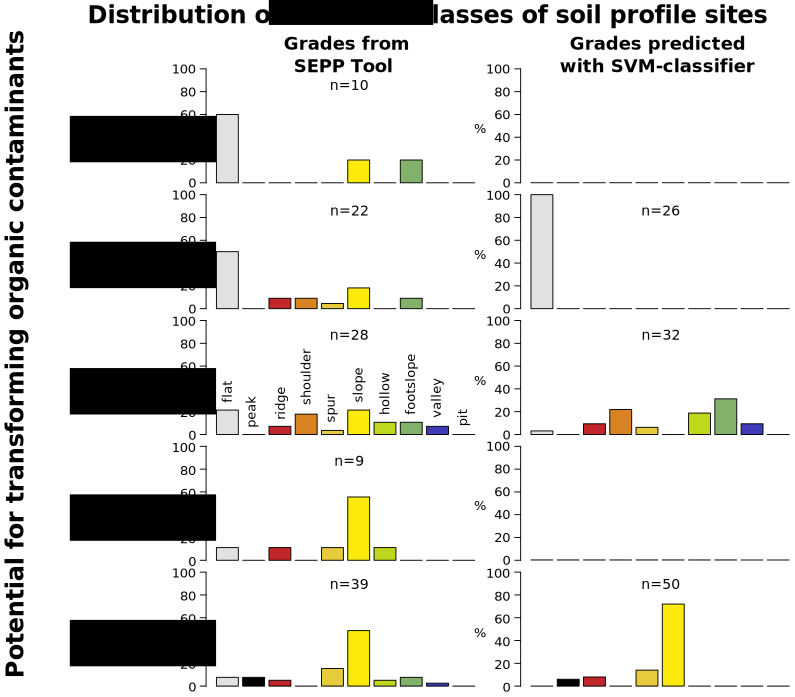
\includegraphics[width=\textwidth,angle=0]{landforms_transformorganic.pdf}
\caption{Barplots representing the distribution of the landform classes for the different grades regarding the potential to transform organic contaminants. The left column shows the distribution for the original set of grades as evaluated by the SEPP tool, where the right column shows the distribution of the grades as awarded by the SVM-classifier based on landforms and maximal curvature.}
\label{fig:transformorganic}
\end{figure}
Together, a model fed with these two parameter leads to a median cross-validated correct classification rate of 46.3~\%. It predicts the grades 2, 3, and 5, with the majority of class 1 soils being misclassified as grade 3, and all but two of the grade 4 soils as incorporated into the class with grade 5.
\subsection{Potential as  filter and buffer for organic contaminants}
The distribution of this potential over the study area is very one-sided, with all but four soil profiles evaluated as belonging to the class with the poorest potential. As a consequence, modeling this potential is not very productive, as the classifiers will simply classify the four soils with grade 4 as grade 5, which still leads to the high correct classification rate of 96~\%.
\subsection{Potential for retention of water-soluble contaminants}
The most dominant grade for potentially retaining water-soluble contaminants such as nitrate is grade 1, with 47 soil profiles. Grades 2 and 3  are similar with 14 and 17 member, followed by a slight peak in member ship for grade 4 with 22 profile sites. As the climatic framework is the same for the study area, this potential is basically evaluted using soil texture. A SVM-classifier applying high resolution slope and minimum curvature leads to a median cross validated accuracy of 53.7. Due to its dominance in the original data,  the predicted class grade 1, which the model links to very low slope angles and minimum curvature values not far away from zero, incorporates a large number of soil profiles with different grades, leading to a very high user's accuracy of 96~\%, but also a producer's reliability of only 60~\%. The model predicts all classes except for grade 2, however grades 3 and 5 are projected for only two soils each, with grade 3 producing a user's accuracy of only 12~\%. The reason for this can be identified in the  box plot analysis, which shows that for these 2 smaller classes the classifying algorithm concentrates on outliers in order to produce significant differences to the distribution of the relevant terrain parameters of the other classes.
\subsection{Potential as buffer for acidic contaminants}
Soils with the highest potential are the most numerous in the study area, constituting 36~\% of all profile sites. With decreasing potential, the membership numbers also decrease, with only 9 soils attributed with the lowest potential by the SEPP tool. Planar curvature and slope, both computed with the high resolution (2.5~m) DTM and local-scale window size of 12.5~m, result in a model with a median accuracy of 48.1~\%. A major drawback of this model is that with regard to the result based on the majority vote of 100 model runs, it fails to reproduce any members of the classes with grade 2 and 5. While the small sample size may be an issue for grade 5, 83~\% of the soils originally with grade 2 are  fitted into the predicted grade 1, as these classes share a very similar terrain parameter distribution for both slope and curvature.  Grades 3 and 4 are distinguishable by increasingly higher slope and also planar curvature values.



 \section{Discussion}
Some of the algorithms implemented in SEPP, such as the one responsible for calculating the grades for the potential for agricultural production, apply thresholds directly related terrain parameters such as slope. As a consequence, these cut-off values are immediately detected by the SVM classifier  and therefore used in its model. This may have the negative effect that the less dominant influence of other topographic factors or landforms on the calculation of this potential is overprinted by the effect of this threshold value and cannot even me mitigated by the addition of further terrain parameters to the model.

The analysis of the SVM classifier predicting average precipitation retention capacity highlights the problem of outliers in the distribution.

A large part of the models lead to separation of the study area into two topographically different regions. On the one hand only gently sloping area of the paleovalley, and on the other the steeper slopes to the east and west. This is also well in line with the different land uses, as the former represents the area which is used for agricultural purposes, while the latter is mainly covered with forest. The potential as a CO2 sink shows similar issues!
 
Using less classes, as is the case for the potential to provide nutrients for plants, may be more appropriate when searching for general trends with regard to the influence of topography on the evaluation of soil functions.

Prediction of the potentials proved best for the soil functions....


Problem with bimodal distributions leads to the prediction of only a limited number of classes.

sampling

Important for model evaluation to see if the class where misclassifications occure is "far" away from the correct class.

SVM classification was preferred to other statistical models, for instance logistic regression, for its smooth predictions \citep{Steger2016} when applied as a spatial predictor.SVM are used as an exploratory tool here. Analysis of predictions with more predictor variables has shown a decrease in cross validated error due to overfitting with increasing number of explanatory variables.


\section{Conclusions}

xxx


\vspace{6pt} 

%%%%%%%%%%%%%%%%%%%%%%%%%%%%%%%%%%%%%%%%%%
%% optional
%\supplementary{The following are available online at \linksupplementary{s1}, Figure S1: title, Table S1: title, Video S1: title.}

% Only for the journal Methods and Protocols:
% If you wish to submit a video article, please do so with any other supplementary material.
% \supplementary{The following are available at \linksupplementary{s1}, Figure S1: title, Table S1: title, Video S1: title. A supporting video article is available at doi: link.}

%%%%%%%%%%%%%%%%%%%%%%%%%%%%%%%%%%%%%%%%%%
\authorcontributions{For research articles with several authors, a short paragraph specifying their individual contributions must be provided. The following statements should be used “conceptualization, X.X. and Y.Y.; methodology, X.X.; software, X.X.; validation, X.X., Y.Y. and Z.Z.; formal analysis, X.X.; investigation, X.X.; resources, X.X.; data curation, X.X.; writing—original draft preparation, X.X.; writing—review and editing, X.X.; visualization, X.X.; supervision, X.X.; project administration, X.X.; funding acquisition, Y.Y.”, please turn to the  \href{http://img.mdpi.org/data/contributor-role-instruction.pdf}{CRediT taxonomy} for the term explanation. Authorship must be limited to those who have contributed substantially to the work reported.}

%%%%%%%%%%%%%%%%%%%%%%%%%%%%%%%%%%%%%%%%%%
\funding{
This research was performed within the project 'Terrain Classification of ALS Data to support Digital Soil Mapping', funded by the Autonomous Province Bolzano -- South Tyrol (Grant nr. 15/40.3).}

%%%%%%%%%%%%%%%%%%%%%%%%%%%%%%%%%%%%%%%%%%
\acknowledgments{We would like to thank Hannes Kleindienst?}

%%%%%%%%%%%%%%%%%%%%%%%%%%%%%%%%%%%%%%%%%%
\conflictsofinterest{The authors declare no conflict of interest. The funders had no role in the design of the study; in the collection, analyses, or interpretation of data; in the writing of the manuscript, or in the decision to publish the results.} 

%%%%%%%%%%%%%%%%%%%%%%%%%%%%%%%%%%%%%%%%%%
%% optional
\abbreviations{The following abbreviations are used in this manuscript:\\

\noindent 
\begin{tabular}{@{}ll}
SVM & Support Vector Machine\\
DTM & Digital Terrain Model\\
CV & Cross validation

\end{tabular}}

%%%%%%%%%%%%%%%%%%%%%%%%%%%%%%%%%%%%%%%%%%
%% optional
\appendixtitles{no} %Leave argument "no" if all appendix headings stay EMPTY (then no dot is printed after "Appendix A"). If the appendix sections contain a heading then change the argument to "yes".
\appendixsections{multiple} %Leave argument "multiple" if there are multiple sections. Then a counter is printed ("Appendix A"). If there is only one appendix section then change the argument to "one" and no counter is printed ("Appendix").
\
%%%%%%%%%%%%%%%%%%%%%%%%%%%%%%%%%%%%%%%%%%
% Citations and References in Supplementary files are permitted provided that they also appear in the reference list here. 



% The following MDPI journals use author-date citation: Arts, Econometrics, Economies, Genealogy, Humanities, IJFS, JRFM, Laws, Religions, Risks, Social Sciences. For those journals, please follow the formatting guidelines on http://www.mdpi.com/authors/references
% To cite two works by the same author: \citeauthor{ref-journal-1a} (\citeyear{ref-journal-1a}, \citeyear{ref-journal-1b}). This produces: Whittaker (1967, 1975)
% To cite two works by the same author with specific pages: \citeauthor{ref-journal-3a} (\citeyear{ref-journal-3a}, p. 328; \citeyear{ref-journal-3b}, p.475). This produces: Wong (1999, p. 328; 2000, p. 475)

%=====================================
% References, variant B: external bibliography
%=====================================
\externalbibliography{yes}
\bibliography{P3}


%% for journal Sci
%\reviewreports{\\
%Reviewer 1 comments and authors’ response\\
%Reviewer 2 comments and authors’ response\\
%Reviewer 3 comments and authors’ response
%}

%%%%%%%%%%%%%%%%%%%%%%%%%%%%%%%%%%%%%%%%%%
\end{document}

